\documentclass[hidelinks]{article}
\usepackage[utf8]{inputenc}
\usepackage{blindtext}
\usepackage[parfill]{parskip} % for flush indenting
\usepackage{amsmath, amsfonts, amsthm, amssymb, centernot, siunitx} % math symbols
\usepackage{hyperref, cleveref}
\usepackage{geometry}
\usepackage{graphicx}
\usepackage{txfonts}
\usepackage{listings}
\usepackage{color}

\definecolor{dkgreen}{rgb}{0,0.6,0}
\definecolor{gray}{rgb}{0.5,0.5,0.5}
\definecolor{mauve}{rgb}{0.58,0,0.82}

\lstset{frame=tb,
  language=R,
  aboveskip=3mm,
  belowskip=3mm,
  showstringspaces=false,
  columns=flexible,
  basicstyle={\small\ttfamily},
  numbers=none,
  numberstyle=\tiny\color{gray},
  keywordstyle=\color{blue},
  commentstyle=\color{dkgreen},
  stringstyle=\color{mauve},
  breaklines=true,
  breakatwhitespace=true,
  tabsize=3
}

\geometry{a4paper,
left=30mm,
right=30mm,
top=30mm}
\linespread{1.2}

\newtheoremstyle{break}
{\topsep}{\topsep}%
{\upshape}{}%
{\bfseries}{}%
{\newline}{}%
\theoremstyle{break}
\renewcommand{\section}[2]{\theoremstyle{break} \newtheorem*{thm#1}{#1}\begin{thm#1}#2\end{thm#1}}

\date{April 13, 2023}
\author{\texttt{Names Removed}}
\title{%
Real Estate Valuation Data Set Analysis }


\begin{document}
\maketitle
\newpage
\section{Introduction}{Real estate is a crucial component of any economy, serving as both an asset and a key driver of economic growth. The value of real
estate is determined by a variety of factors, including location, condition, and demand. Analyzing the factors that contribute to
the value of real estate and the growth of that value can provide insights into the economic health of a region and inform
investment decisions. The Real Estate Valuation Data Set provides a rich source of information for studying the factors that
influence the value of real estate. The data set includes information on the sale price (in NT\$10000 per ping, where 1 ping is
equal to 3.3 squared meters) of real estate properties in Taiwan, as well as a variety of features such as the age of property (in
years), the distance to the nearest MRT station (in meters), the number of convenience stores in the surrounding area, as well as
location data (longitude and latitude in degrees). The data set also includes information on the transaction date, allowing for
temporal analysis of real estate trends. This project aims to analyze the Real Estate Valuation Dataset to provide investment
advice on where in the region to purchase real estate based on which factors of real estate in this region are associated with
higher growth in price over time. We will do this by engineering many variables and interactions, and investigating which
variables, when multiplied by date, are useful predictors of price, as this would indicate which properties may be worth more when
sold in the future.
}
\section{Location characterization}{Since we are interested in the difference between rural and urban homes, we need to be able to classify homes as either rural or
urban. By using prominent dividing features of the district like rivers and major roads we divided the location into two regions,
urban and rural as seen in \cref{fig:regions}. We now consider the distributions of ppua (price per unit area) for rural and urban
homes separately. Looking at \cref{fig:boxplot} we see that the homes with the highest ppua are predominately urban while still
being atypical compared to other urban homes. This \textit{could} be explained by noting that certain types of properties, such as
luxury apartments which have high ppua, are expected to be more common in urban neighborhoods than rural ones while still being
relatively uncommon overall. Regardless of the explanation, it makes sense to transform ppua by taking the logarithm so that these
outlier values don't influence our models and interpretations disproportionately. For the remainder of this paper, ppua will refer
to log-transformed ppua. As a final note, the ppua of urban homes appears to be noticeably higher on average than that of rural
homes as seen in \cref{fig:ppuamap}.}
\section{Trends in the data}{We now seek any other relationships between the explanatory variables and the response variable ppua. Consider first the effect of
the sell month on ppua. Looking at \cref{fig:seasonal} it appears that ppua may fluctuate according to a sinusoidal pattern. But
with that said we have rather limited data, spanning a period of only 12 months and looking at the mean ppua
(\cref{fig:seasonalmean}) does not reveal any pattern whatsoever. So although it is probably still worth exploring how seasonality
affects ppua when fitting our models we should interpret results pertaining to the seasonality with a grain of salt.

At first glance it would appear that the age of a house has a quadratic relationship with ppua. But after separating the data into
urban and rural, we see that both groups show a linear relationship between age and ppua. See \cref{fig:age}. The reason that when
viewed together the data may have appeared quadratic is because rural homes decay in ppua faster than urban homes do with respect
to age, so the lines intersect to form a $v$ shape.

Yet again the initial look is deceptive when looking at \cref{fig:mrt} which appears exponential in nature. However once divided
into rural and urban groups we have a linear relationship with a small slope for urban homes, but still what seems like an
exponential relationship for rural homes. One possible explanation for this difference is that the shape really is exponential but
urban areas will have more MRT stations than rural areas over a smaller footprint and so most homes will be closer to an MRT
station and over this range of distances the relationship looks linear. Some rural homes may happen to be close to an MRT station
but most of them will be farther away spread out across a larger area, allowing us capture the full shape. The fact that we took
the log-transform of ppua does in fact help with this.

When urban and rural properties are taken together there is a linear trend of moderate positive slope between the number of nearby
convenience stores and ppua, see \cref{fig:stores}. When separated, the relationship becomes almost a constant one for urban homes
while for rural homes the linear trend becomes more pronounced. This makes sense for similar reasons as the results about MRT
stations made sense. Notice however that even for rural houses there is little difference between the ppua of houses with between
2 and 4 convenience stores. This could be explained by the fact that being close to 3 stores isn't practically any better than
being close just 2 stores. Distance to the closest store may be a more useful feature. Perhaps the jump in ppua seen in
rural home after being close to 5 or more stores is an artifact of having little data on these types of houses.

The fact that patterns keep emerging in the data when we split into the urban and rural categories is a good sign that we did a
good job of location characterization. It also worth noting that there are no obvious relationships between any two of the
explanatory variables.
}
\section{Model Selection}{To determine the optimal number of variables to include in our model, we performed both forward and backward selection to
determine which variable count range consistently performed well on different tests. We tested using three criteria: Mallow`s Cp,
Bayesian Information Criteria, and the Adjusted R-Squared. A benefit of using forward/backward selection is that potential
colinearity between features will be implicitly handled since redundant features get discarded.

The best variable count according to Mallow`s Cp is where the variable count is both close to the Mallow`s Cp value and is small.
Consulting \cref{fig:mallowcp} we see that with forward selection a variable count of 9 as the smallest Cp value and its
Cp value is 8.605 which is relatively close to 9, and with backward selection a variable count of 9 is the best because it
has a Cp value of 8.542. Although a variable count of 10-15 have smaller Cp values for backward selection, their Cp values are not
very close to their respective variable counts which makes these variable counts not as optimal. Both forward and backward
selection suggest that 9 variable counts is optimal.

The best variable count according to BIC is the variable count with the smallest BIC value. According to \cref{fig:bic}, with
forward selection a variable count of 7 has the smallest BIC. While with backward selection a variable count of 8 has the smallest
BIC value. In general, a variable count of 7-8 seems to be optimal for the BIC test.

The best value for Adjusted R-Squared is the variable count with the largest Adjusted R-Squared value. Consulting \cref{fig:rsq}
with forward selection a variable count of 17 has the largest Adjusted RSQ. Conversely, with backward selection a variable count
of 14 has the largest Adjusted RSQ. Since forward and backward selection yielded different results, it is inconclusive whether 14
or 17 is the best variable count. According to both figures, it appears that any variable count greater than 8 seems to have a
good adjusted R-Squared.

Overall, we would say that a variable count of 7-9 seems to consistently produce a good result according to the three criterias.
To pick a variable count which is sound, we performed cross validation with variable counts of 7-9 and selected the
variable count with the lowest Root Mean Squared Error (RMSE). After performing the cross validation, a variable count of 9 is selected.
The summary for our best model is shown in \cref{fig:summary}.
}
\newpage
\section{Leverage and Influence}{After selecting our model, we inspect the absolute residuals (see \cref{fig:standres}) to check for outliers. There is one obvious
outlier which, referring back to the price map, is very cheap compared to its neighbours. The nature of the sale may have been
different. For instance, the buyer may have been in a hurry to sell, or it could have been a transaction between family or
friends. To determine what influence this outlier may have had on the model, we created maps for leverage values as well as Cook's
distances (see \cref{fig:cook} and \cref{fig:lev}), and these metrics do not suggest that the extreme outlier had much influence.
Notice in \cref{fig:lev} that the properties with the greatest leverage tend to be quite far away from other properties. With
access to more data it may be reasonable to consider a three class split between urban/suburban/rural.

In addition to the extreme outlier, however, there are 5 other moderate outliers (defined as having absolute standardized residual
greater than three) which do align to points in the graph having more influence. We repeated the model selection process, and
found that while the forward/backward selection step yielded similar results after removing outliers, the final model selected
could vary slightly. However, the general conclusion on which features were relevant did not change much. The best models found
after removing outliers are summarized in \cref{fig:n=413} and \cref{fig:n=408}.

% \begin{verbatim}

% Call:
% lm(formula = as.formula(paste("log(price) ~", paste(show.best.variables(subset,
% 	variable.count), collapse = "+"))), data = full.df.train)

% Residuals:
%  	Min   	1Q   Median   	3Q  	Max
% -0.52200 -0.11056  0.00297  0.08976  0.80362

% Coefficients:
%                   	Estimate Std. Error t value Pr(>|t|)    
% (Intercept)     	-5.476e+02  1.230e+02  -4.453 1.17e-05 ***
% date             	2.737e-01  6.108e-02   4.481 1.03e-05 ***
% age             	-1.086e-02  2.046e-03  -5.309 2.07e-07 ***
% mrt             	-8.240e-05  1.344e-05  -6.133 2.53e-09 ***
% stores           	5.487e+01  2.442e+01   2.247  0.02533 *  
% `date:is.urban`  	2.474e-04  3.715e-05   6.660 1.19e-10 ***
% `age:is.urban`   	4.854e-03  2.293e-03   2.116  0.03509 *  
% `mrt:date:is.urban` -8.755e-08  2.785e-08  -3.144  0.00182 **
% `stores:date`   	-2.722e-02  1.213e-02  -2.244  0.02550 *  
% `stores:is.urban`   -5.232e-02  1.155e-02  -4.529 8.38e-06 ***
% ---
% Signif. codes:  0 ‘***’ 0.001 ‘**’ 0.01 ‘*’ 0.05 ‘.’ 0.1 ‘ ’ 1

% Residual standard error: 0.185 on 321 degrees of freedom
% Multiple R-squared:  0.769,    Adjusted R-squared:  0.7625
% F-statistic: 118.7 on 9 and 321 DF,  p-value: < 2.2e-16








% Call:
% lm(formula = as.formula(paste("log(price) ~", paste(show.best.variables(subset,
% 	variable.count), collapse = "+"))), data = full.df.train)

% Residuals:
%  	Min   	1Q   Median   	3Q  	Max
% -0.49132 -0.09697  0.00571  0.09669  0.61094

% Coefficients:
%                   	Estimate Std. Error t value Pr(>|t|)    
% (Intercept)      	3.406e+00  5.547e-02  61.406  < 2e-16 ***
% age             	-1.466e+01  4.023e+00  -3.645 0.000312 ***
% mrt             	-6.593e-02  4.794e-02  -1.375 0.170032    
% `date:is.urban`  	2.618e-04  3.440e-05   7.611 3.13e-13 ***
% `age:date`       	7.279e-03  1.998e-03   3.643 0.000315 ***
% `age:is.urban`   	4.772e-03  2.121e-03   2.250 0.025165 *  
% `mrt:date`       	3.270e-05  2.381e-05   1.373 0.170632    
% `mrt:date:is.urban` -7.481e-08  2.456e-08  -3.046 0.002514 **
% `stores:date`    	3.736e-05  4.765e-06   7.840 6.92e-14 ***
% `stores:is.urban`   -6.479e-02  1.072e-02  -6.041 4.29e-09 ***
% ---
% Signif. codes:  0 ‘***’ 0.001 ‘**’ 0.01 ‘*’ 0.05 ‘.’ 0.1 ‘ ’ 1

% Residual standard error: 0.1665 on 317 degrees of freedom
% Multiple R-squared:  0.8218,    Adjusted R-squared:  0.8167
% F-statistic: 162.4 on 9 and 317 DF,  p-value: < 2.2e-16

% \end{verbatim}
}
\section{Conclusion}{Our analysis of the real estate valuation data set revealed that the growth rate of property values is higher in urban areas
compared to rural areas. It's worth mentioning that although the response variable is simply price per unit area, most of the
explanatory variables in our model are interacting with the date variable allowing us to capture growth in real estate value over
time. This finding suggests that investing in real estate in urban can yield a higher return on investment in the long run.
Furthermore, our analysis showed that properties located closer to public transit systems in urban areas experience higher growth
rates compared to those that are farther away. This observation could be attributed to the convenience and accessibility provided
by public transit systems, making it easier for people to access job opportunities and amenities, thus increasing the demand for
properties in those areas. Therefore, investing in properties close to public transit systems in urban areas could be a viable
strategy for real estate investors looking to maximize their returns. On the other hand, we also found that distance-related
features such as distance to the nearest MRT station, distance to the nearest convenience store, and distance to the city center,
were less important in rural areas compared to urban areas. This may be because people living in rural areas are more likely to
have their own cars and rely less on public transportation. Thus, the demand for properties in rural areas may be influenced by
other factors such as the availability of natural resources, access to good schools, and quality of life. Overall, our analysis
highlights the importance of location and accessibility to public transportation in the real estate market. Investing in urban
areas close to public transit systems could offer higher returns, while investing in rural areas may require a different set of
consideration. 
}
\newpage
\section{Figures}{See the relevant figures below.
% Maps
\begin{figure}[hbt!]
    \centering
    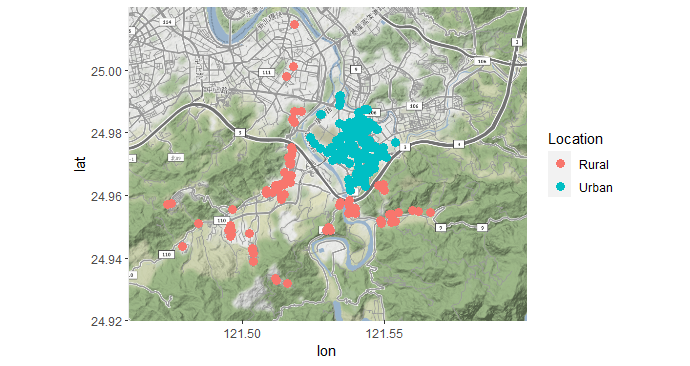
\includegraphics[scale=0.80]{img/regions.png}
    \caption{Xindian District divided into regions}
    \label{fig:regions}
\end{figure}

\begin{figure}[hbt!]
    \centering
    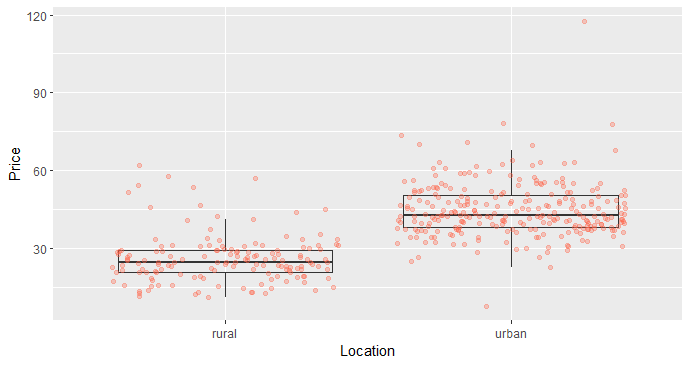
\includegraphics[scale=0.75]{img/boxplot.png}
    \caption{(non log) ppua distributions by location}
    \label{fig:boxplot}
\end{figure}

\begin{figure}[hbt!]
    \centering
    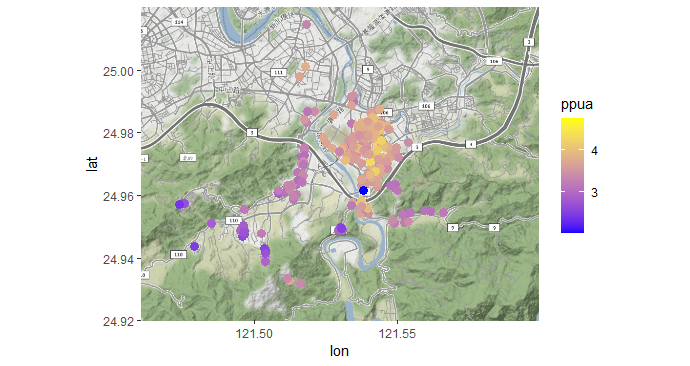
\includegraphics[scale=0.80]{img/ppuamap.png}
    \caption{Xindian district by ppua}
    \label{fig:ppuamap}
\end{figure}

% Seasonal
\begin{figure}[hbt!]
    \centering
    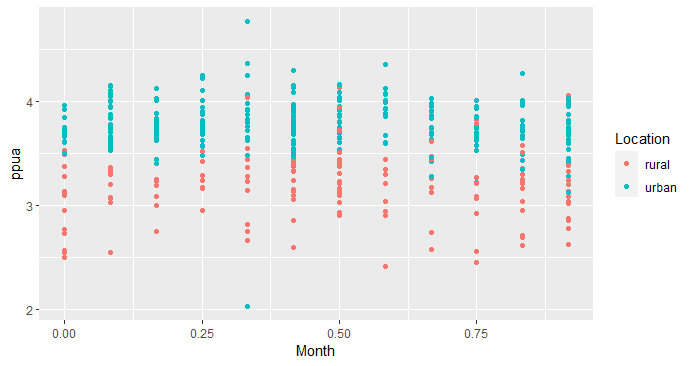
\includegraphics[scale=0.80]{img/seasonal.png}
    \caption{ppua by month}
    \label{fig:seasonal}
\end{figure}

\begin{figure}[hbt!]
    \centering
    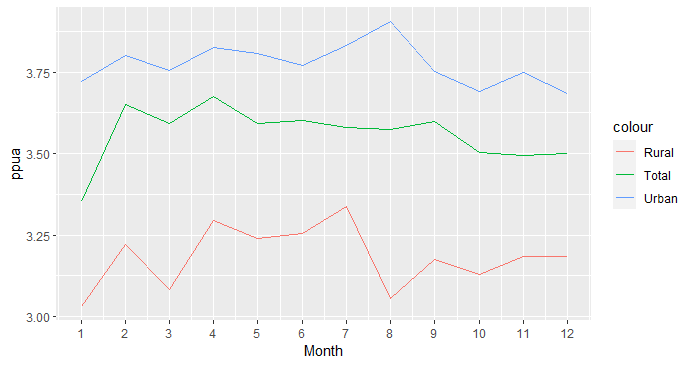
\includegraphics[scale=0.80]{img/seasonalmean.png}
    \caption{mean ppua by month}
    \label{fig:seasonalmean}
\end{figure}

% Age
\begin{figure}[hbt!]
    \centering
    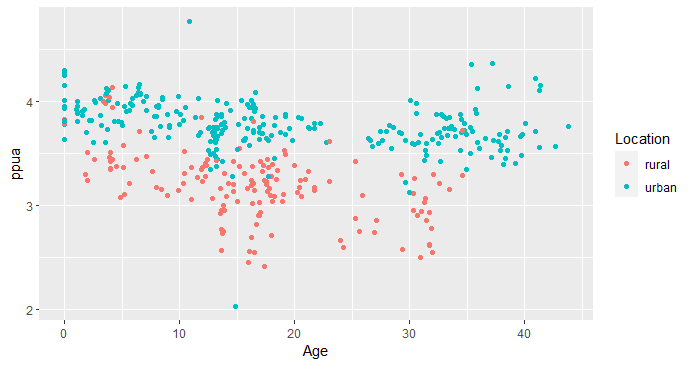
\includegraphics[scale=0.80]{img/agetogether.png}
    \caption{ppua vs age}
    \label{fig:age}
\end{figure}

% \begin{figure}[ht]
%     \centering
%     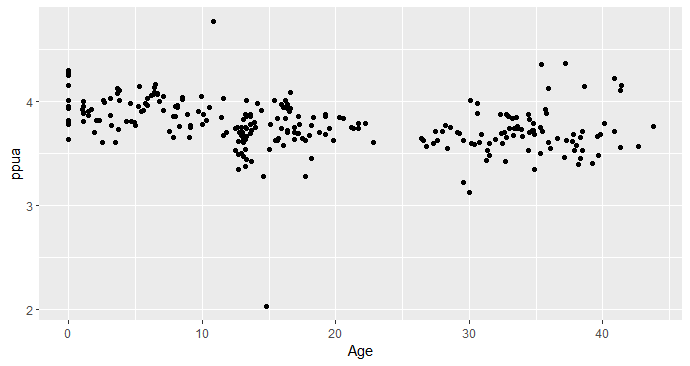
\includegraphics[scale=0.80]{img/ageurban.png}
%     \caption{ppua vs age for urban homes}
%     \label{fig:ageurban}
% \end{figure}

% \begin{figure}[ht]
%     \centering
%     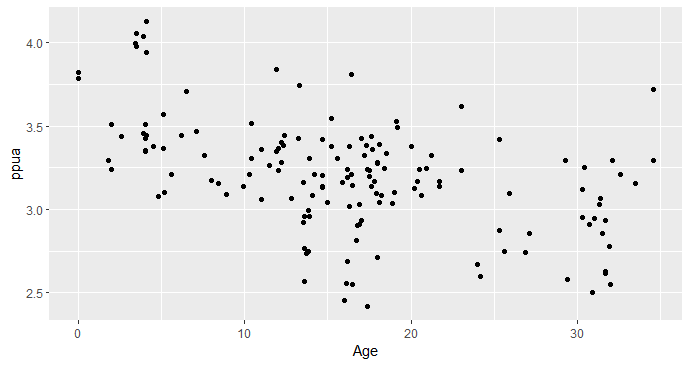
\includegraphics[scale=0.80]{img/agerural.png}
%     \caption{ppua vs age for rural homes}
%     \label{fig:agerural}
% \end{figure}

% MRT
\begin{figure}[hbt!]
    \centering
    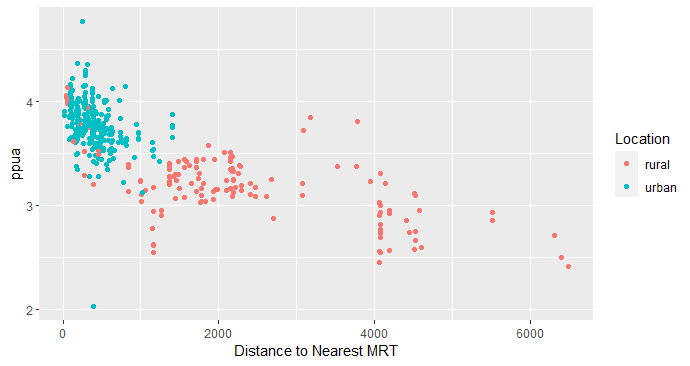
\includegraphics[scale=0.80]{img/mrttogether.png}
    \caption{ppua vs distance to the near mrt}
    \label{fig:mrt}
\end{figure}

% \begin{figure}[ht]
%     \centering
%     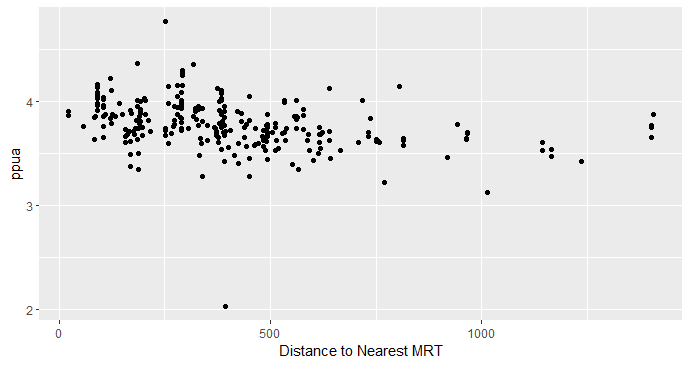
\includegraphics[scale=0.80]{img/mrturban.png}
%     \caption{ppua vs distance to the near mrt for urban homes}
%     \label{fig:mrturban}
% \end{figure}

% \begin{figure}[ht]
%     \centering
%     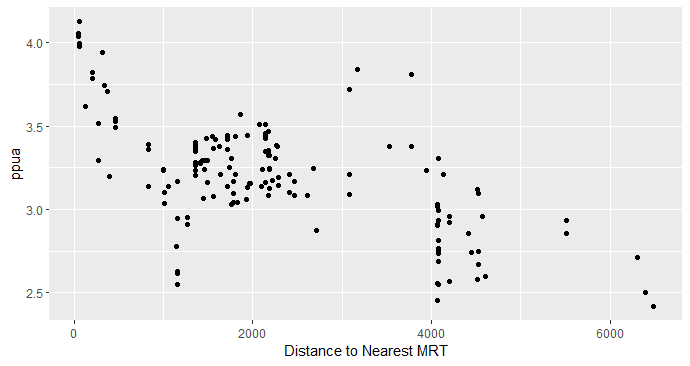
\includegraphics[scale=0.80]{img/mrtrural.png}
%     \caption{ppua vs distance to the near mrt for rural homes}
%     \label{fig:mrtrural}
% \end{figure}

% Stores 
\begin{figure}[hbt!]
    \centering
    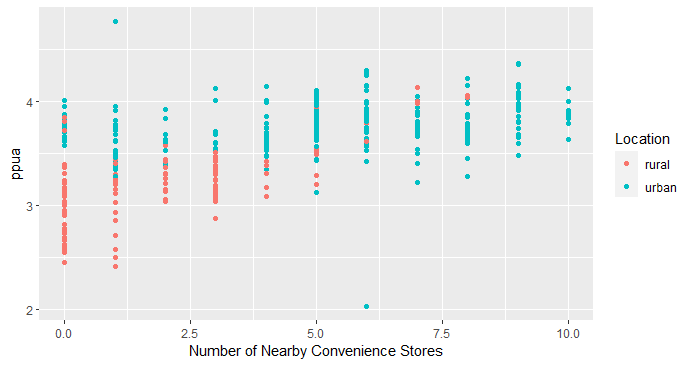
\includegraphics[scale=0.80]{img/storestogether.png}
    \caption{ppua vs number of nearby convenience stores}
    \label{fig:stores}
\end{figure}

% \begin{figure}[ht]
%     \centering
%     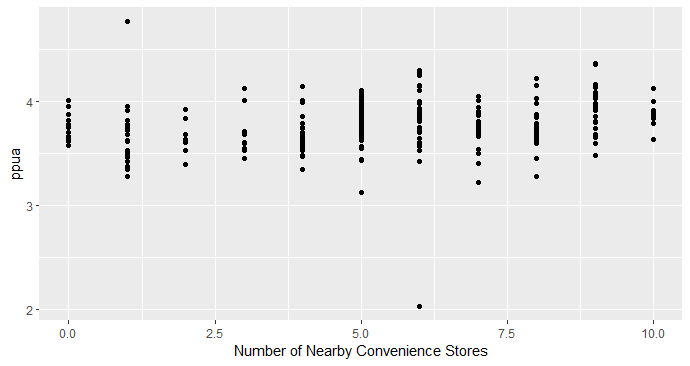
\includegraphics[scale=0.80]{img/storesurban.png}
%     \caption{ppua vs number of nearby convenience stores for urban homes}
%     \label{fig:storesurban}
% \end{figure}

% \begin{figure}[ht]
%     \centering
%     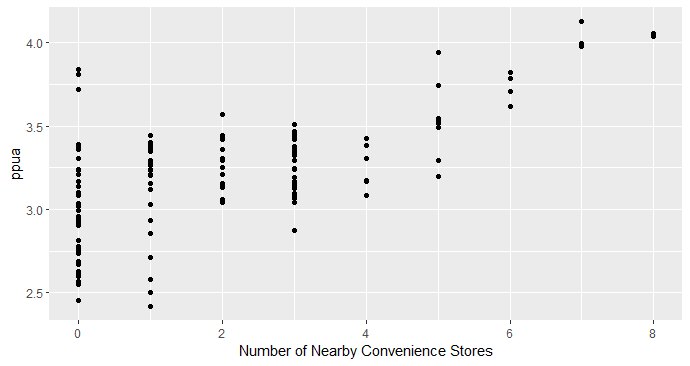
\includegraphics[scale=0.80]{img/storesrural.png}
%     \caption{ppua vs number of nearby convenience stores for rural homes}
%     \label{fig:storesrural}
% \end{figure}

\begin{figure}[hbt!]
    \centering
    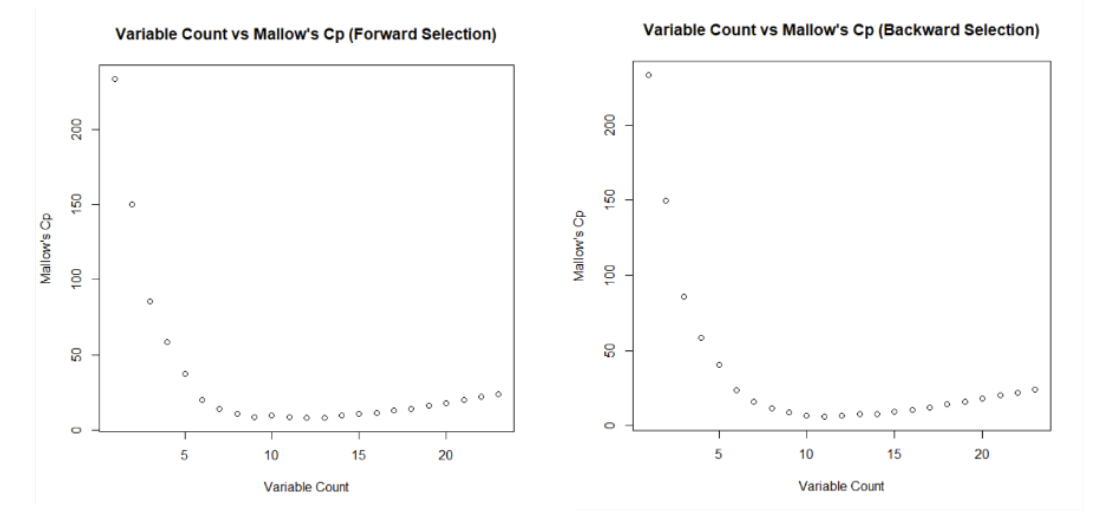
\includegraphics[scale=0.34]{img/mallowcp.png}
    \caption{Mallow's Cp for forward and backward selection}
    \label{fig:mallowcp}
\end{figure}

\begin{figure}[hbt!]
    \centering
    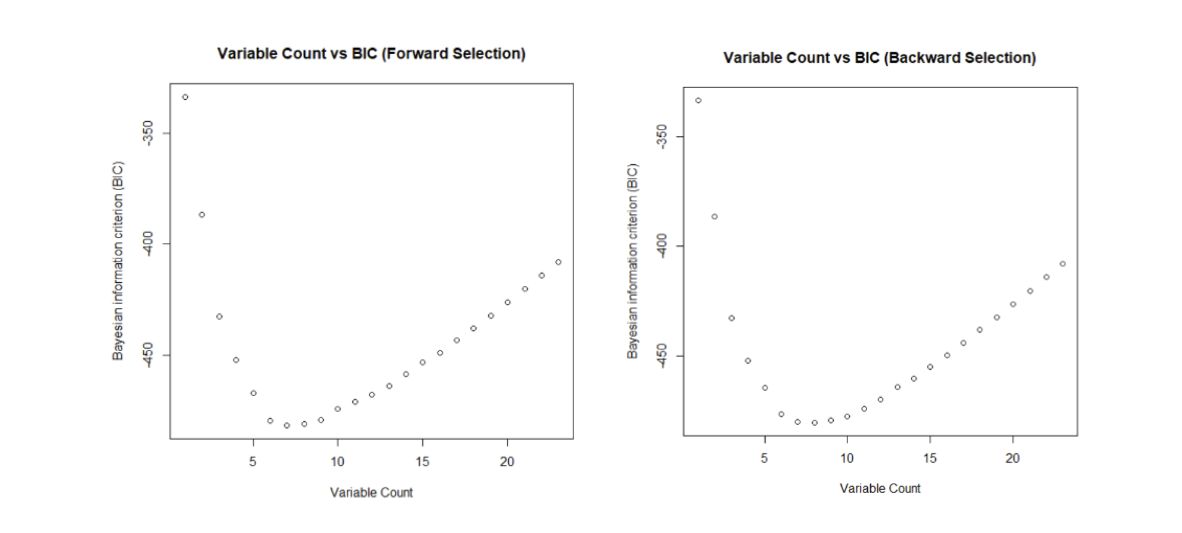
\includegraphics[scale=0.35]{img/bic.png}
    \caption{BIC for forward and backward selection}
    \label{fig:bic}
\end{figure}

\begin{figure}[hbt!]
    \centering
    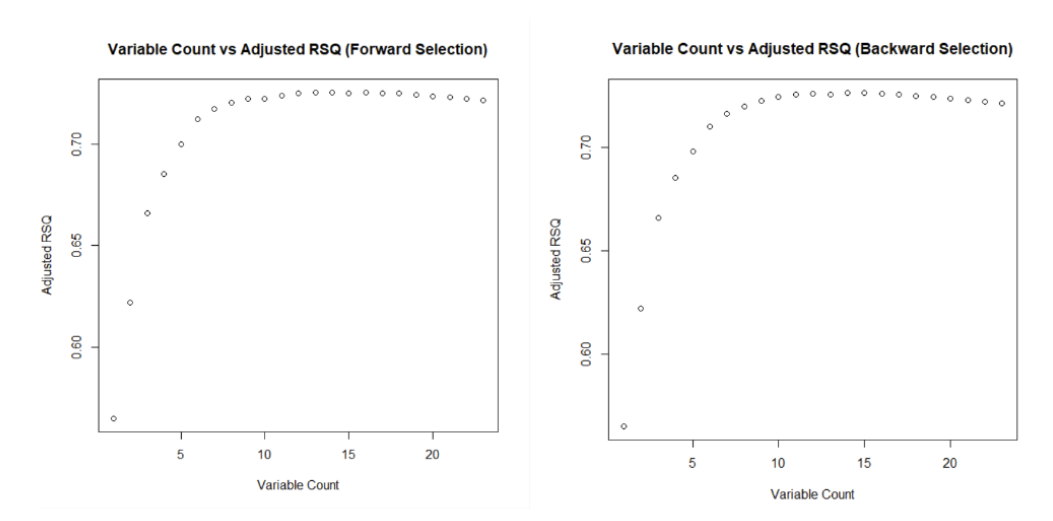
\includegraphics[scale=0.37]{img/rsq.png}
    \caption{Adjusted $R^2$ for forward and backward selection}
    \label{fig:rsq}
\end{figure}

\begin{figure}[hbt!]
    \centering
    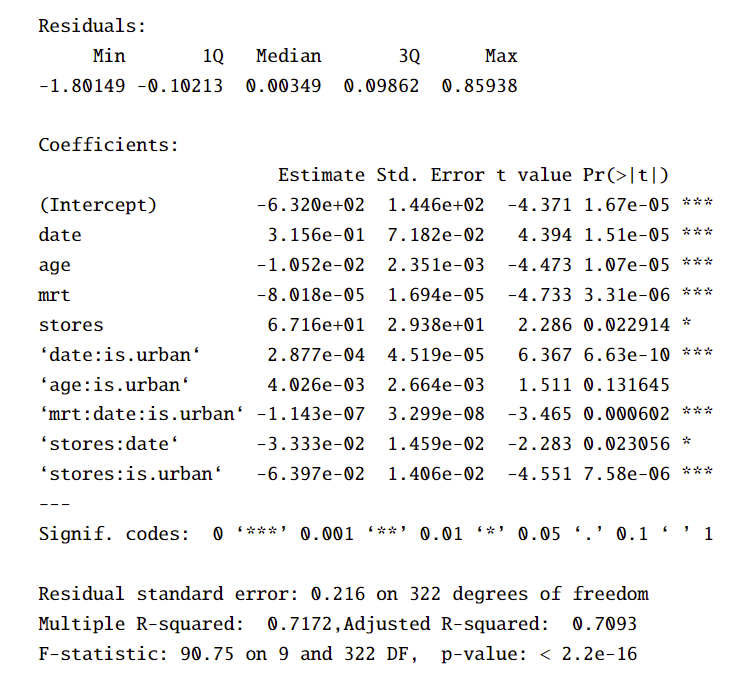
\includegraphics[scale=0.7]{img/summary.png}
    \caption{Summary of the best model}
    \label{fig:summary}
\end{figure}

\begin{figure}[hbt!]
    \centering
    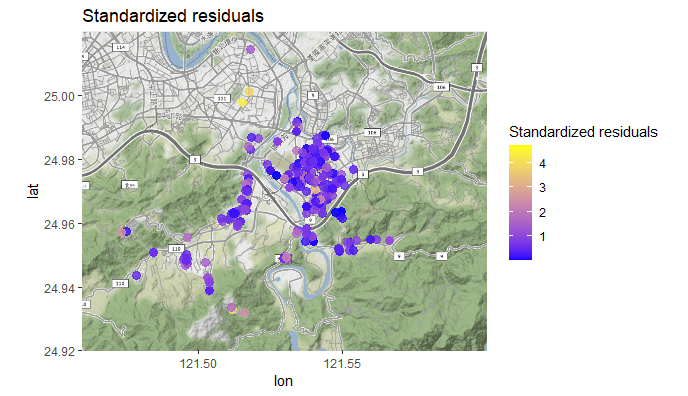
\includegraphics[scale=0.80]{img/standres.png}
    \caption{Standardized residuals}
    \label{fig:standres}
\end{figure}

\begin{figure}[hbt!]
    \centering
    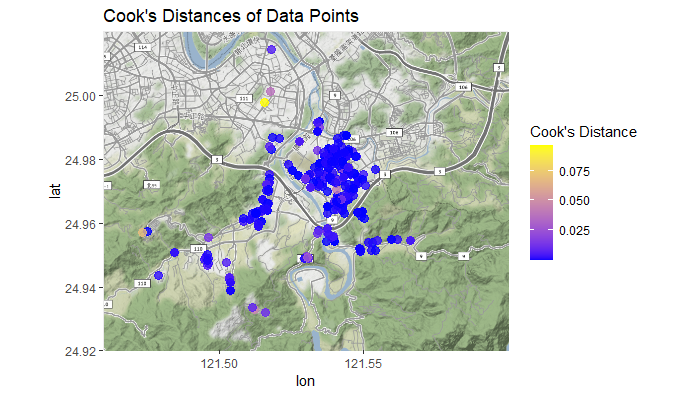
\includegraphics[scale=0.80]{img/cook.png}
    \caption{Cook's distance}
    \label{fig:cook}
\end{figure}

\begin{figure}[hbt!]
    \centering
    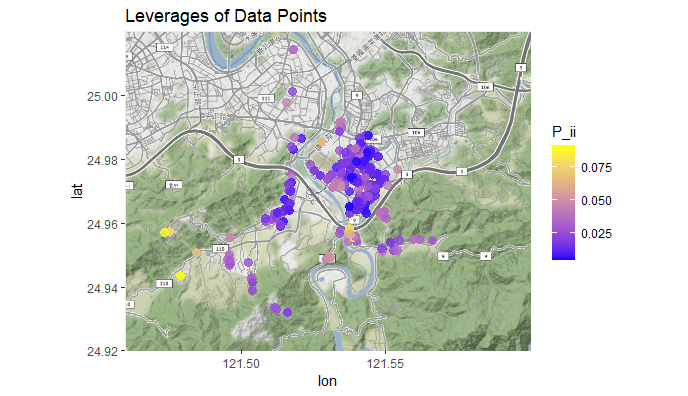
\includegraphics[scale=0.80]{img/lev.png}
    \caption{Leverage}
    \label{fig:lev}
\end{figure}

\begin{figure}[hbt!]
    \centering
    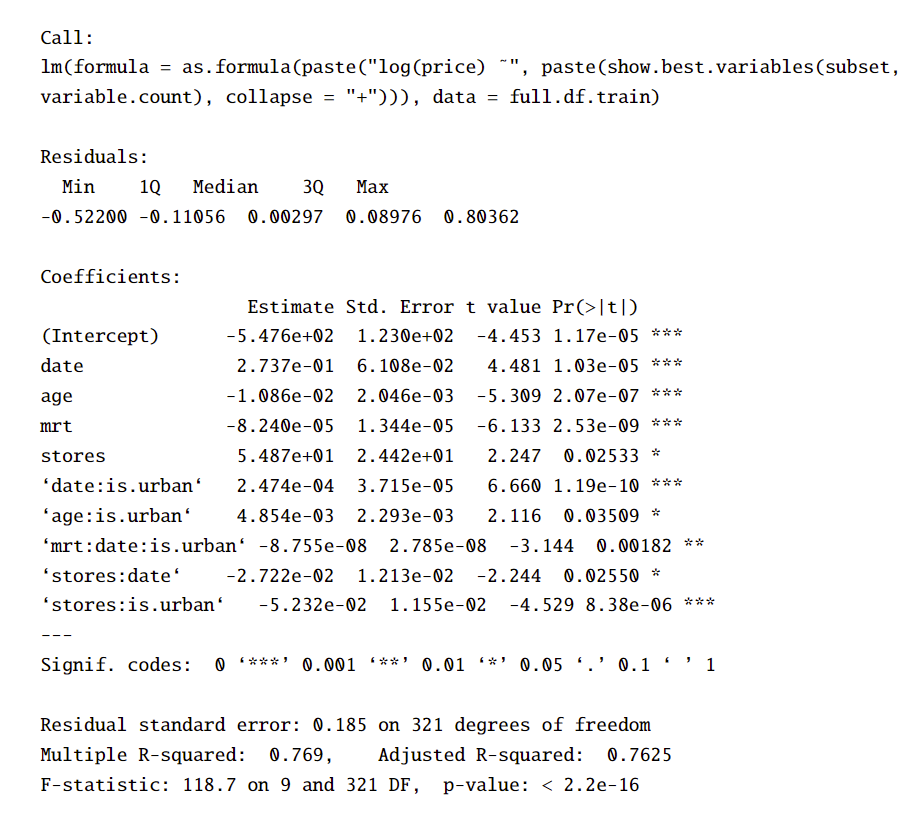
\includegraphics[scale=0.65]{img/n=413.png}
    \caption{Summary of the best model after removing the most extreme outliers}
    \label{fig:n=413}
\end{figure}

\begin{figure}[hbt!]
    \centering
    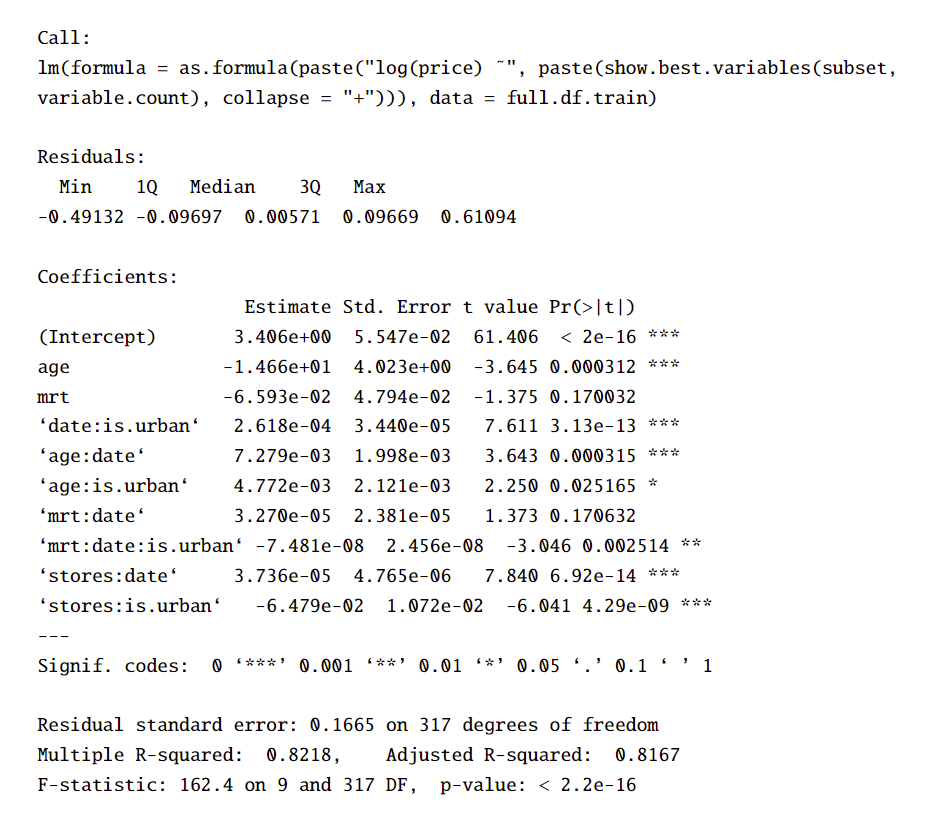
\includegraphics[scale=0.65]{img/n=408.png}
    \caption{Summary of the best model after removing all outliers}
    \label{fig:n=408}
\end{figure}

\clearpage }
% \newpage
% \section{R Script}{\input{r.tex}}
\end{document}